\chapter{Introduction} % 1 page max
\label{ch:Introduction}


\section{Context and objective}
\label{sec:Contexte}

\textbf{Quantum computing} is a rapidly expanding field. This technology, which enables qubits to be manipulated instead of the bits that form the basis of today's computing, paves the way for algorithms that are more powerful than conventional ones. As the quantum machines running these algorithms are still under development and costly, there is a need for tools to simulate and verify quantum algorithms using classical machines. The aim of this project is to propose a model of the data structure of abstract additive quantum decision diagrams, based on existing work, and to simulate them in order to study their performance.


\section{State of the art}
\label{sec:Etat}


\subsubsection*{Quantum computing}

The first postulate of quantum physics, the \textbf{principle of superposition}, states that the state space of a quantum system is a Hilbert space. Consequently, while a \textit{bit} can classically only be in a $\ket 0$ or $\ket 1$ state, its quantum counterpart, the \textbf{qubit}, can be in a superposition of these two states.
$$\ket \psi = \alpha \ket 0 + \beta \ket 1$$

\noindent where $\alpha, \beta$ are complex coefficients. The second postulate, the \textit{measurement principle}, states that when a qubit is measured, it is projected onto one of the base states $\ket 0$ or $\ket 1$ with probability $|\alpha|^2$ or $|\beta|^2$ respectively.

States with $n$ qubits can be represented by $2^n$-dimensional \textbf{vectors}, the states of the set consisting of two systems being those obtained by tensor product (\textit{Kronecker product}) of a state of the first system and a state of the second. It is this exponential number of complex parameters for a multi-qubit state that makes the classical study of quantum algorithms difficult, since the states take up exponentially large amounts of memory.

\vspace{1em}

As in classical computing, elementary operations on memory are performed in quantum computing by \textbf{gates}. From a mathematical point of view, a gate operating on $n$ qubits is commonly represented by a matrix of size $2^n \times 2^n$. Applying a gate $M$ to a set of qubits $v$ then amounts to multiplying the state vector by the gate matrix.

Parallel application of multiple gates to multiple qubits is represented by the \textbf{tensor product} (Kronecker product) of the gate matrices. It should be noted, however, that the application of gates to qubits in this way takes exponential time as a function of the number of qubits, making the naive use of quantum algorithms on classical machines inefficient.

The application of gates to qubits is frequently represented as \textbf{quantum circuits}, where qubits are represented by lines and gates by boxes.

\begin{figure}
  \centering
  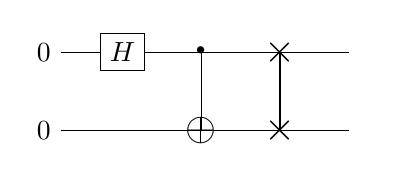
\begin{tikzpicture}
    \node (end1) at (4, 0) {};
    \node (end2) at (4, -1) {};
    \node (q1) at (0, 0) {$\ket 0$};
    \node (q2) at (0, -1) {$\ket 0$};

    \node [draw] (h1) at (1, 0) {$H$};
    \draw (q1) -- (h1);
    \draw (h1) -- (end1);
    \draw (q2) -- (end2);
    \node (cx) at (2, -1) {\Large $\oplus$};
    \node (cx2) at (2, 0) {\Huge $\cdot$};
    \node (s1) at (3, 0) {\Large $\times$};
    \node (s2) at (3, -1) {\Large $\times$};

    \draw (s1.center) -- (s2.center);
    \draw (cx2.center) -- (cx.center);
  \end{tikzpicture}
  \caption{2-qubits circuit with gates $H$, $CX$ and $S$}
\end{figure}

Any \textit{unitary} and \textit{reversible} matrix can be used as a quantum gate. Among the most common gates are the Hadamard gate ($H$), the “not” gate ($X$), the “controlled not” gate ($CX$), or the swap gate ($S$). These and other gates are used in quantum algorithms such as Deutsch-Josza's \cite{DJ_1992}, Grover's \cite{Grover_1996} and Shor's \cite{Shor_1997}.

\vspace{1em}

To provide a unified language for developing quantum algorithms from gates that can be interpreted on any hardware, IBM released the \textbf{Open QASM} programming language in 2017. \cite{QASM_2017} It defines qubits on which gates are applied, and the program can then be simulated or executed on a quantum computer as on a conventional computer. The preceding circuit can, for example, be represented by the program \ref{lst:QASM}:

\begin{figure}[thp]
  \renewcommand{\figurename}{Program}
  \centering
\begin{tabular}{c}
\begin{lstlisting}
  qubit a;
  qubit b;
  h a;
  cx a b;
  s a b;
\end{lstlisting}
\end{tabular}
\caption{Example Open QASM code}
\label{lst:QASM}
\end{figure}

\subsubsection*{Decision diagrams}

The \textbf{decision diagram} structure is a data structure developed in the 1970s. It has since become widely used in computer science, in particular to make the representation of binary functions more compact.

Take, for example, the binary function $f(x_1, x_2, x_3) = x_1 \lor (x_2 \land x_3)$. In the general case, such a function is represented using a \textit{truth table}, i.e. in a size that grows exponentially with the number of binary variables considered. A more compact representation can be achieved using a decision diagram, as shown in \autoref{fig:ExempleDD}, where left-hand children are indicated by dotted arrows and right-hand children by solid arrows.

\begin{figure}
  \renewcommand{\arraystretch}{0.8}% Tighter
  \begin{tabular}{c|c|c|c}
    $x_1$ & $x_2$ & $x_3$ & $f(x_1, x_2)$ \\
    \hline
    0 & 0 & 0 & 0 \\
    0 & 0 & 1 & 0 \\
    0 & 1 & 0 & 0 \\
    0 & 1 & 1 & 1 \\
    1 & 0 & 0 & 1 \\
    1 & 0 & 1 & 1 \\
    1 & 1 & 0 & 1 \\
    1 & 1 & 1 & 1
  \end{tabular}
  \hfill{}
  % https://tikzcd.yichuanshen.de/#N4Igdg9gJgpgziAXAbVABwnAlgFyxMJZAJgBoAGAXVJADcBDAGwFcYkQAPAfQEYACADoDGEAE58AFN2KDh9MFD7cAzAEoQAX1LpMufIRTLSy6nSat2PTdpAZseAkXIVTDFm0QgpvdVp339J1IeV3MPL2lfGzs9RxRnYlD3dm81a39Yg2QeYySLT3J0210HLJyQmjd8zi4ZIUZ5RRUimNKiMkTKsPZmjVMYKABzeCJQADNRCABbJGcQHAgkADYaRiwwcKh6OAALAaKJ6dmaBaQckAAjGAUkZTmq8O5+AF4+Kz8QQ5nEFfnFxAArKt1pttnsoCAuslPNJnoVVvQrowAAolQKeURYQY7HAHSbfX6nRAAdih1Vh7xsXyQpL+SCBIDWG3YW12+zJjy4yj4r0KH2pJJO-3ODx6XOe70oGiAA
  \begin{tikzcd}[column sep=tiny]
    (x_1) &                                                                & x_1 \lor (x_2 \land x_3) \arrow[ld, dashed] \arrow[rddd, "x_1 = 1", bend left] &   \\
    (x_2) & x_2 \land x_3 \arrow[dd, "x_2=0"', dashed] \arrow[rd, "x_2=1"] &                                                                                &   \\
    (x_3) &                                                                & x_3 \arrow[ld, "x_3 = 0", dashed] \arrow[rd, "x_3=1"]                          &   \\
          & 0                                                              &                                                                                & 1
    \end{tikzcd}
    \hfill{}
  % https://tikzcd.yichuanshen.de/#N4Igdg9gJgpgziAXAbVABwnAlgFyxMJZARgBoAGAXVJADcBDAGwFcYkQQBfU9TXfQigBMpAMzU6TVu2JceIDNjwEi5MRIYs2iEOTm8lA1aWIap2jtwP8VKMkLNb2XCTCgBzeEVAAzAE4QALZIaiA4EEiiNIxYYBZQ9HAAFm76IP5BITThSGQgAEYwYFCR5FbpAcGIUWERiCIgMXHsCcmp0fSFjAAKfMqCIH5Y7kk4aRlVNTmIACzlE0gz2XUNTfGJKSXzlYvLuZyUnEA
  \begin{tikzcd}[column sep=huge, row sep=large]
    & {} \arrow[ld, dashed] \arrow[rddd, bend left] &   \\
  {} \arrow[dd, dashed] \arrow[rd] &                                               &   \\
    & {} \arrow[ld, dashed] \arrow[rd]              &   \\
  0                                &                                               & 1
  \end{tikzcd}

  \caption{(a) Table de vérité (b) Diagramme de décision (c) Diagramme de décision sans labels}
  \label{fig:ExempleDD}
\end{figure}

Decision diagrams take advantage of the data's internal \textbf{structure} (here, a Boolean function). On the one hand, labels are not needed to reconstruct the values taken by the function.
On the other hand, in the worst case, i.e. where the function has no structure allowing reduction, the size of the decision diagram (its number of branches) is $2^{n+1} - 2$ which, like the number of values $2^n$ to be stored in a truth table, is \textbf{exponential} in $n$. In the worst case, decision diagrams offer no improvement, but are not asymptotically worse than truth tables either.

\subsubsection*{Abstract interpretation}

Abstract interpretation is a general method of dealing with the properties of computer programs by abstracting them. It was introduced by Patrick and Radhia Cousot in 1977 \cite{CousotCousot77-1}. It can also be used to solve problems or compute faster.

Consider the following problem: we're trying to determine the sign of the expression $-12 \times 7 - 13$. We could calculate the result of this expression, but we could also note that $-12$ and $-13$ are negative and that 7 is positive, hence $-12 \times 7$ is negative, so the expression is negative. More formally, we've taken the concrete elements $-12$, 7 and $-13$ and replaced them with the abstract elements $\oplus$ “positive” and $\ominus$ “negative”, on which we define sum and product operations according to well-known rules.

There are many uses for the abstract interpretation \cite{Rosendahl_1995}, for example in program compilation. In this project, we'll be using it to reduce quantum decision diagrams, even if this means losing some of the information they contain. This is also the case for the previous example: abstracting elements by their sign does not always allow us to determine the sign of the expression.


\section{Contribution}
\label{sec:Contribution}

The various concepts presented in the state of the art can all be used to improve the computation speed or memory size of a dataset. The aim of this project was therefore to combine these concepts, adding an extra dimension, additivity: the fact that a diagram has several right (respectively left) wires, the interpretation being that the “effective right wire” is the sum of the diagram's right (respectively left) wires.
The aim of the project was therefore to propose a model of abstract, additive quantum decision diagrams, and to simulate them in order to study their performance in comparison with other models.

As a preliminary step, a study of polar complex intervals was carried out, which had not been done in the literature until now.
A mathematical \textbf{model} of the data structure and reduction methods were formalized, and reduction algorithms were developed to reduce these diagrams.
In addition, methods for applying quantum gates to the diagrams have been formalized.
An \textbf{implementation} of these algorithms was carried out, without relying on existing libraries (except for unit tests).

\section{Structure of the report}
\label{sec:Structure}

\autoref{ch:Modele} presents the theoretical model of quantum decision diagrams that has been developed, including the accompanying reduction and gating algorithms. Next, \autoref{ch:Implementation} discusses the implementation carried out. Finally, a short conclusion is presented in \autoref{ch:Conclusion}.

A more complete theoretical document is available online. Some theoretical points succinctly presented in this report, or theorems whose proof is not specified, are detailed in this document. \cite{Leroy_2025} In addition, technical documentation of the code is available online. \cite{Leroy_doc}
